
\chapter{Invasion Percolation: Fractal-based Search Diversification}


\section{Breadth-Based Diversification:\\ Invasion Percolation}
\label{sec:ip}
\subsubparagraph{intro}

A limitation of  type-based diversification based on path distance % path dist estimates are included in in ``based on path dist''
is that it does not diversify with respect to breadth -- 
nodes with equal estimated distance from goals ($h$), initial states ($g$) or plateau entrance ($d$) are put in a single set.
This makes it susceptible to pathological behavior on graphs where some nodes have many more children than others.

\begin{figure}[hbt]
 \centering
 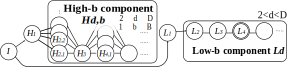
\includegraphics{img/model3.pdf}
 \caption{Example case exhibiting large bias in the branching factor depending on the subgraph.}
 \label{fig:model}
\end{figure}

Consider a blind search on the directed acyclic graph
shown in \refig{fig:model}.
The graph consists of two large components, \textbf{high-b} and \textbf{low-b} branches, and their entries $H_1,L_1$. The initial search node is $I$ and the goal node is $L_4$.
Both branches have maximum depth $D$, and the high-b branch has maximum width $B$.
Both $B$ and $D$ are very large.
This graph presents a pathological case for all of the previously described methods (\lifo, \fifo, \ro and type-based diversification), depending on successor ordering.
\lifo performs a DFS, and if \lifo first searches $H_1$ and the high-b branch due to successor ordering, it must explore the entire high-b branch before expanding $L_1$ and low-b branch.
\fifo performs Breadth-First Search (BreadthFS), and  will therefore suffer from the  high branching factor at depth 2 of the high-b branch, getting stuck before reaching $L_4$.
Although randomization can allow \ro to be better off than the behavior of \fifo/BreadthFS, the effect is limited:
For example, while expanding depth 2, \ro may occasionally expand depth 3 because it uniformly randomly selects a node from OPEN.
However, the probability of expanding nodes at depth 3 is initially only $1/(B+1)$ and continues to be small until  most of the nodes at depth 2 are expanded, 
because OPEN is mostly populated with the nodes from depth 2.
Depth-based diversification addresses the depth bias of BreadthFS.
However, even though it distributes the effort among various depths,
the probability of expanding $L_2,L_4$ at depths 2 and 4, is only $1/(B+1)$ each, which is very low when $B$ is very large.

We propose \;\emph{Invasion Percolation-based diversification (IP-diversification)}, a new diversification strategy for satisficing search that addresses this type of bias.
% in \refig{fig:model} for satisficing planning,%not limited to planning
% As discussed above, a diversification scheme seeks to allocate resources evenly among a group of nodes in order to avoid undesirable biases.
% One approach to implementing diversification is to treat diversification in a search graph as the problem of evenly covering the graph over time.
% By considering the graph as a multidimensional lattice, we can apply techniques that have been developed for modeling percolation in multidimensional lattices.
IP-diversification combines randomization and Prim's method \cite{prim1957shortest} for Minimum Spanning Tree (MST).
% -- we seek an unbiased method for evenly exploring a search graph based on this model.
